\chapter{Results and summary}
\label{Chap4}
\section{Results \& statistical interpretations}
\label{sec:results}

The background predictions described in Section~\ref{sec:bkgestimation} are 
summed together for the final statistical SMS interpretations. Each analysis
bin is represented as a individual counting experiment with one 
signal process and five background processes.  Each process is assumed 
to be a Poisson distribution with some number of prior distribution representing
the uncertainty on the corresponding process's rate parameter. The exact
details of how these uncertainties are modeled depends on the 
details of each of the background estimation methods that were used. 

In general, each background estimation is a scaling of a Poisson process 
from a control region, $N^{\mathrm{pred}}_{\mathrm{bkg}}=N^{\mathrm{pred}}_{\mathrm{CR}}\beta$, where $\beta$ 
is the transfer factor, $N^{\mathrm{pred}}_{\mathrm{CR}}$ is the expected yield in the 
control region of the corresponding process, and $N^{\mathrm{pred}}_{\mathrm{bkg}}$ is the 
prediction provided as the expected mean of the corresponding process's
Poisson distribution for a given signal region.  In general,  $N^{\mathrm{pred}}_{\mathrm{CR}}$
is constrained by the observed yields in the control region, 
$N^{\mathrm{obs}}_{\mathrm{CR}}$ and there are five such constraints from each 
of the 5 control regions discussed in Section~\ref{sec:bkgestimation}.  For a 
simplified counting experiment with only one background process and one signal
process, the likelihood for this type of background prediction would be, 

\begin{equation}
\centering
\mathcal{L}(N^{\mathrm{pred}}_{\mathrm{sig}},N^{\mathrm{pred}}_{\mathrm{bkg}}|N^{\mathrm{obs}}_{\mathrm{SR}},N^{\mathrm{obs}}_{\mathrm{CR}}) \propto \left(N^{\mathrm{pred}}_{\mathrm{bkg}}+N^{\mathrm{pred}}_{\mathrm{sig}}\right)^{N^{\mathrm{obs}}_{\mathrm{SR}}}e^{-N^{\mathrm{pred}}_{\mathrm{bkg}}}\cdot\left(\frac{N^{\mathrm{pred}}_{\mathrm{bkg}}}{\beta}\right)^{N^{\mathrm{obs}}_{\mathrm{CR}}} e^{-N^{\mathrm{pred}}_{\mathrm{bkg}}/\beta}
\end{equation}

This likelihood, is equivalent to a Poisson likelihood with a gamma distribution
as the prior and can be used to constrain both the predicted background the 
signal strength in the signal region with the proper modeling of the $N^{\mathrm{pred}}_{\mathrm{bkg}}$ 
uncertainty due to limited statistics of the control region observed yield.

As such, we modeling the uncertainty on the prediction due to limited 
control region statistics as a gamma distribution.  This procedure is followed, especially when the 
observed control region statistics are too small to justifying a Gaussian 
approximation.  While the observed control region events vary considerably, 
for the signal regions in extreme corners of our phase space the use of a 
Gamma prior distribution is critical for modeling uncertainties.  For uniformity, 
we generally use it everywhere.  The exception to this, as mentioned below, is 
the $e$+jets control region, 
which is used for estimating the fake-photon background, where we use a Gaussian prior 
to model the effect of limited control region statistics.  Note, the number of 
observed events in these control regions is always larger than 17 events, for 
which the $1\sigma$ intervals of a Poisson distribution and Gaussian distribution
still agree to within ~10\%.  

The uncertainty on the transfer factors used to scale the observed event yields 
in the control regions are modeled with log-normal prior
distributions.  These priors account for uncertainties typically arising 
from limited MC statistics, systematic effects do to composition or limited knowledge 
of object reconstruction efficiencies, or PDF/scale uncertainties.  Uncertainties 
from limited MC statistics are typically uncorrelated across each of the 
search regions.  Other source of systematic uncertainty typically correlate 
expected yields from various signal regions.  Details of the modeling of 
systematic uncertainties for each of the background estimations is given below. 

For the lost-e and lost-$\mu+\tau_{\mathrm{had}}$ predictions, the uncertainties
on the prediction are modeled with a gamma distribution, with the 
shape parameter set to the observed number of events in the corresponding
$\ell-\gamma$ control region and the scale parameter is set to be the
average transfer factor, given in Table~\ref{tab:lost_lepton_SF}.  There 
are also log-normal prior distributions used to model the uncertainties
of the transfer factors, which account for:

\begin{itemize}
 \item limited MC statistics; the corresponding nuisance parameters are fully uncorrelated.
 \item PDF and scale uncertainties; the corresponding nuisance parameters are fully correlated across signal regions and between lost-e and lost-$\mu+\tauh$.
 \item jet energy scale uncertainties; the corresponding nuisance parameters are fully correlated across all signal regions.
 \item lepton scale factor uncertainties; the corresponding nuisance parameters are fully correlated across \ptmiss bins and fully uncorrelated across \nb, \nj regions;
 \item uncertainties related to soft/collinear photon modeling; the corresponding nuisance parameters are fully correlated
 for lost-e and negligible for $\mu+\tau_{\mathrm{had}}$ prediction.
 %\item b-tagging scale factor uncertainties
\end{itemize}
For the fake-rate estimation of $W+\gamma$ and $t\bar{t}+\gamma$ events, the systematic uncertainties
from the control region statistics are typically small.  All of the uncertainties
are modeled with log-normal prior distributions whose uncertainties
correspond to:

\begin{itemize}
 \item the statistical uncertainty from the $e\rightarrow\gamma$ control regions; the corresponding nuisance parameters are fully uncorrelated across all signal regions.
 \item fake rate scale factors; the corresponding nuisance parameters are fully correlated across all signal regions.
 \item uncertainties due to pileup and initial state radiation (ISR) modeling of simulations; the corresponding nuisance parameters are fully correlated across all signal regions.
\end{itemize}

For the Z$\gamma$ predictions, the statistical uncertainties from control 
region are modeled with a gamma
prior distribution whose shape parameter is the observed events in the 
$Z(\ell\ell)\gamma$ control region and the scale parameter is the 
purity-corrected MC transfer factor, which in the nomenclature of 
Equation~\ref{eq:zgamma} is 
$\beta\cdot N_{\nu\nu+\gamma}^{\mathrm{MC}}/N_{\ell\ell+\gamma}^{\mathrm{MC}}$.
Additional log-normal prior distributions are included to account 
for
\begin{itemize}
 \item the effect of limited MC statistics on $N_{X+\gamma}^{\mathrm{MC}}$; the corresponding nuisance parameters are fully uncorrelated across all signal regions;
 \item uncertainties on the purity; the corresponding nuisance parameter fully correlates the effect across all signal regions.
 \item uncertainties due to b-tag scale factors; the corresponding nuisance parameters are fully correlated across \ptmiss and \nj bins, anti-correlated across \nb regions.
 \item uncertainty due to missing higher order corrections; the corresponding nuisance parameters are fully correlated across \ptmiss bins, uncorrelated across \nb, \nj regions.
\end{itemize}


For the multijet predictions, the systematic uncertainties due to limited 
control region statistics are modeled with a 
Gamma prior distribution whose shape parameter is the observed number
of events in the low-$\dphi$ control regions and the scale parameter
is the product of the high-to-low ratio, $R_{\mathrm{h/l}}$, the double ratio
correction factors, $\kappa$, and the purity, $\beta$, obtained from data-driven predictions
of the electroweak backgrounds in the low-$\dphi$ control regions. 
Systematic uncertainties on the knowledge of this combined transfer factor are 
modeled with log-normal prior distributions and account for

\begin{itemize}
 \item uncertainties on $R_{\mathrm{h/l}}$ due to limited number of events in data sideband; the corresponding nuisance parameters 
 are fully correlated across \ptmiss bins and fully uncorrelated across \nb, \nj regions.
 \item uncertainties on $\kappa$ based on validations with zero photon events; the corresponding nuisance parameters are fully 
   correlated across \ptmiss bins and fully uncorrelated across \nb and \nj regions.
 \item uncertainties on $\beta$ due to all uncertainties as described above; the corresponding nuisance parameters are 
  fully uncorrelated across all search regions.
\end{itemize} 

All of the uncertainties associated with the signal yields, described in detail
in Section~\ref{sec:signal-systematics}, are modeled with log-normal prior distributions.  
Nuisance parameters associated with ISR modeling uncertainties are correlated 
across the various \nj bins, but uncorrelated across \nb and \ptmiss regions.  
Nuisance parameters associated with \ptmiss modeling in simulation are
correlated across the various \ptmiss bins and uncorrelated across \nb and 
\nj regions.  Nuisance parameters associated with b-tagging scale factors are fully correlated
across all \ptmiss and \nj, but anti-correlated across the \nb regions. The nuisance 
parameters associated with the statistical uncertainties of our simulated samples
are fully uncorrelated across all signal regions. A single nuisance parameter
is associated with the luminosity uncertainty and fully correlates the effect
across all signal regions. 

Expected and observed limits are computed after adjusting the central values
and uncertainties associated with all nuisance parameters to data by minimizing 
them with respect to the observed yields while fixing the signal strength to
zero.

The predicted background and observed yields are shown in Table~\ref{tab:finalPrediction} and Fig.~\ref{fig:summaryPlot}.
The largest deviation is found in bin 2 ($2\leq\nj\leq 4$, $\nb=0$, and $270<\ptmiss<350\ \gev$), where the background is predicted to be 91 events
with 51 events observed.
The local significance of this single bin was computed to be around 2 standard deviations below the SM expectation.
This calculation does not account for the look-elsewhere effect associated with the use of 25 exclusive signal regions,
which is expected to reduce this significance.
In general, a large deviation in a single bin is inconsistent with the expected distributions of events from the signal models considered here.
The observations in all other bins are consistent with the SM expectations within one standard deviation.
\begin{table}[h!]
\tiny
%\renewcommand{\arraystretch}{1.25}
\centering
\caption{Predicted and observed event yields for each of the 25 exclusive signal regions.}
\label{tab:finalPrediction}
\begin{tabular}{cccccccccc}
\nj      & \nb& \ptmiss [GeV]& Lost e              & Lost $\mu$ + \tauh & Misid. $\gamma$   & Z$(\nu\bar{\nu})\gamma$                & \gjets            & Total                 & Data \\
\hline
2--4     & 0  & 200--270     & 10.5 $\pm$ 2.6        & 31.2 $\pm$ 6.0        & 22.3 $\pm$ 5.4 & 33.6 $\pm$ 8.3       & 60   $\pm$ 11         & 157 $\pm$ 16          & 151 \\
2--4     & 0  & 270--350     & 5.8  $\pm$ 1.8        & 29.6 $\pm$ 5.9        & 11.9 $\pm$ 2.9 & 22.9 $\pm$ 6.0       & 20.5 $\pm$ 4.3        & 91  $\pm$ 10          & 51 \\
2--4     & 0  & 350--450     & 1.68 $\pm$ 0.88       & 13.9 $\pm$ 3.9        & 6.6 $\pm$ 1.6  & 17.0 $\pm$ 5.2       & 4.1  $\pm$ 1.4        & 43.3$\pm$ 6.8         & 50 \\
2--4     & 0  & 450--750     & 1.98 $\pm$ 0.94       & 8.1  $\pm$ 3.1        & 6.7 $\pm$ 1.5  & 18.1 $\pm$ 7.1       & 2.5  $\pm$ 1.3        & 37.4$\pm$ 8.0         & 33 \\
2--4     & 0  & ${>}750$     & $0.00_{-0.00}^{+0.69}$& 1.2 $\pm$ 1.2         & 0.79 $\pm$ 0.19& 2.8 $\pm$ 1.2        & $0.41_{-0.41}^{+0.42}$& 5.2 $\pm$ 1.9         & 6 \\
\\ %[\cmsTabSkip]
5--6     & 0  & 200--270     & 1.28 $\pm$ 0.61       & 5.1  $\pm$ 1.9        & 3.53 $\pm$ 0.75& 3.09 $\pm$ 0.78      & 15.8 $\pm$ 4.8        & 28.8 $\pm$ 5.3        & 26 \\
5--6     & 0  & 270--350     & 2.06 $\pm$ 0.80       & 3.2  $\pm$ 1.5        & 2.39 $\pm$ 0.56& 1.98 $\pm$ 0.54      & 3.7  $\pm$ 1.8        & 13.3 $\pm$ 2.6        & 11  \\
5--6     & 0  & 350--450     & 0.77 $\pm$ 0.46       & $0.64_{-0.64}^{+0.65}$& 1.26 $\pm$ 0.30& 1.49 $\pm$ 0.47      & 1.23 $\pm$ 0.97       & 5.4 $\pm$ 1.4         & 8 \\
5--6     & 0  & ${>}450$     & 0.26 $\pm$ 0.26       & 1.9 $\pm$ 1.1         & 1.00 $\pm$ 0.24& 1.65 $\pm$ 0.65      & $0.07_{-0.07}^{+0.52}$& 4.9 $\pm$ 1.4         & 7 \\
\\ %[\cmsTabSkip]
${\geq}7$& 0  & 200--270     & $0.00_{-0.00}^{+0.61}$& $0.0_{-0.0}^{+1.3}$   & 0.72 $\pm$ 0.16& 0.37 $\pm$ 0.11      & 1.8 $\pm$ 1.2         & 2.9 $\pm$ 1.9         & 3 \\
${\geq}7$& 0  & 270--350     & $0.34_{-0.34}^{+0.35}$& 1.5 $\pm$ 1.0         & 0.38 $\pm$ 0.10& 0.24 $\pm$ 0.08      & 1.22 $\pm$ 0.94       & 3.6 $\pm$ 1.5         & 3 \\
${\geq}7$& 0  & 350--450     & $0.34_{-0.34}^{+0.35}$& 0.73 $\pm$ 0.73       & 0.17 $\pm$ 0.05& 0.16 $\pm$ 0.07      & $0.07_{-0.07}^{+0.50}$& 1.46 $\pm$ 0.96       & 0 \\
${\geq}7$& 0  & ${>}450$     & $0.00_{-0.00}^{+0.61}$& $0.0_{-0.0}^{+1.3}$   & 0.20 $\pm$ 0.06& 0.17 $\pm$ 0.08      & $0.00_{-0.00}^{+0.75}$& $0.37_{-0.37}^{+1.60}$& 0 \\
\\ %[\cmsTabSkip]
2--4     & ${\geq}1$  & 200--270     & 3.4  $\pm$ 1.5        & 14.5 $\pm$ 4.2        & 7.1  $\pm$ 1.7 & 3.55 $\pm$ 0.89      & 11.3 $\pm$ 3.3        & 39.8  $\pm$ 5.9       & 50 \\
2--4     & ${\geq}1$  & 270--350     & 2.9  $\pm$ 1.4        & 5.6  $\pm$ 2.5        & 3.79 $\pm$ 0.92& 2.45 $\pm$ 0.65      & 5.7  $\pm$ 1.8        & 20.4  $\pm$ 3.6       & 20   \\
2--4     & ${\geq}1$  & 350--450     & $0.0_{-0.0}^{+1.0}$   & 1.1 $\pm$ 1.1         & 2.00 $\pm$ 0.45& 1.81 $\pm$ 0.55      & 0.59 $\pm$ 0.44       & 5.5  $\pm$ 1.7        & 4  \\
2--4     & ${\geq}1$  & ${>}450$     & 2.3 $\pm$ 1.2         & 4.4 $\pm$ 2.3         & 1.62 $\pm$ 0.38& 2.14 $\pm$ 0.84      & 0.95 $\pm$ 0.54       & 11.5 $\pm$ 2.8        & 8  \\
\\ %[\cmsTabSkip]
5--6     & ${\geq}1$  & 200--270     & 3.5  $\pm$ 1.3        & 2.4  $\pm$ 1.4        & 5.5  $\pm$ 1.2 & 0.76 $\pm$ 0.20      & 7.7  $\pm$ 2.4        & 19.9  $\pm$ 3.3       & 21 \\
5--6     & ${\geq}1$  & 270--350     & 1.06 $\pm$ 0.64       & 4.0  $\pm$ 1.8        & 2.98 $\pm$ 0.63& 0.49 $\pm$ 0.14      & 2.1 $\pm$ 1.0         & 10.6  $\pm$ 2.3       & 15 \\
5--6     & ${\geq}1$  & 350--450     & 0.71 $\pm$ 0.51       & 2.4  $\pm$ 1.4        & 1.38 $\pm$ 0.29& 0.32 $\pm$ 0.11      & $0.30_{-0.30}^{+0.49}$& 5.1 $\pm$ 1.6         & 6   \\
5--6     & ${\geq}1$  & ${>}450$     & $0.35_{-0.35}^{+0.36}$& $0.0_{-0.0}^{+1.4}$   & 0.67 $\pm$ 0.15& 0.48 $\pm$ 0.20      & $0.00_{-0.00}^{+0.56}$& $1.5_{-1.5}^{+1.6}$   & 2 \\
\\ %[\cmsTabSkip]
${\geq}7$& ${\geq}1$  & 200--270     & 0.72 $\pm$ 0.53       & 2.0 $\pm$ 1.2         & 1.68 $\pm$ 0.37& 0.13 $\pm$ 0.04      & 5.9 $\pm$ 5.0         & 10.5 $\pm$ 5.1        & 12 \\
${\geq}7$& ${\geq}1$  & 270--350     & $0.00_{-0.00}^{+0.65}$& 1.33 $\pm$ 0.96       & 0.73 $\pm$ 0.16& 0.10 $\pm$ 0.04      & $0.0_{-0.0}^{+1.1}$   & 2.2 $\pm$ 1.6         & 1 \\
${\geq}7$& ${\geq}1$  & 350--450     & 0.72 $\pm$ 0.53       & $0.0_{-0.0}^{+1.2}$   & 0.44 $\pm$ 0.10& 0.07 $\pm$ 0.03      & $0.0_{-0.0}^{+1.1}$   & $1.2_{-1.2}^{+1.7}$   & 1 \\
${\geq}7$& ${\geq}1$  & ${>}450$     & $0.36_{-0.36}^{+0.37}$& $0.0_{-0.0}^{+1.2}$   & 0.23 $\pm$ 0.07& 0.04 $\pm$ 0.02      & $0.0_{-0.0}^{+1.1}$   & $0.6_{-0.6}^{+1.7}$   & 1 \\
\end{tabular}
\end{table}
\begin{figure}[htb!]
\centering
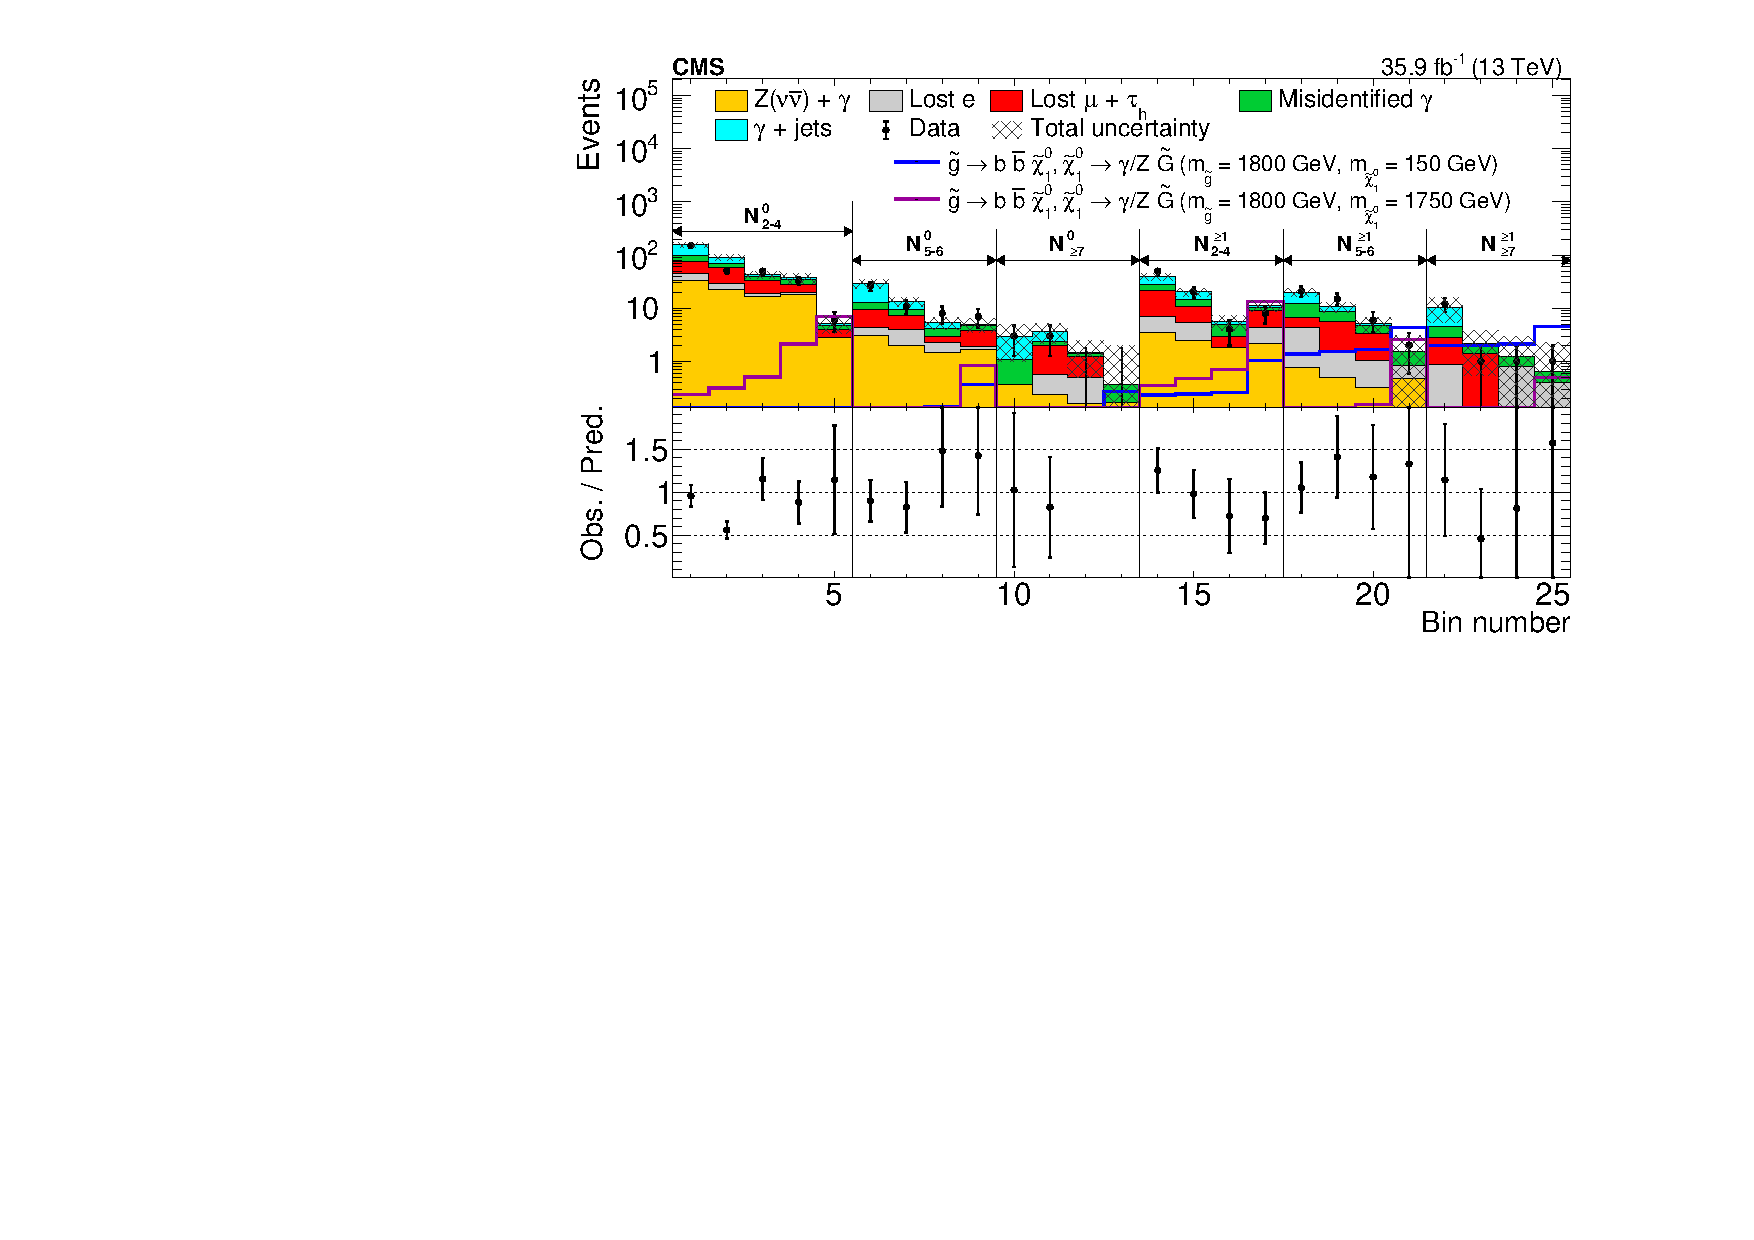
\includegraphics[width=0.99\linewidth]{../Figures/Chap4/Figure_004.pdf}
\captionsetup{width=.95\linewidth}
\caption{Observed numbers of events and predicted numbers of events from the various SM backgrounds in the 25 signal regions.
The categories, denoted by vertical lines, are labeled as \njb,
where j refers to the number of jets and b refers to the number of {\cPqb}-tagged jets.
The numbered bins within each category are the various \ptmiss bins, as defined in Table~\ref{tab:finalPrediction}. The lower panel
shows the ratio of the observed events to the predicted SM background events.
The error bars in the lower panel are the quadrature sum of the statistical uncertainty in the observed data
and the systematic uncertainty in the predicted backgrounds before the adjustments based on
a maximum likelihood fit to data assuming no signal strength.}
\label{fig:summaryPlot}
\end{figure}

The test statistic $q_{\mu} = -2 \ln{\mathcal{L}_{\mu}/ \mathcal{L}_{\mathrm{max}}}$, 
where $\mathcal{L}_{\mathrm{max}}$ 
is the maximum likelihood determined by allowing all parameters, including the signal 
strength, to float, and $\mathcal{L}_{\mu}$
is the profiled likelihood. Limits are determined using the asymptotic form of the test 
statistic \cite{Cowan:2010js} 
in conjunction with the $CL_s$ criterion \cite{Junk1999,bib-cls}. Expected 
upper limits are derived by varying observed yields according to expectations from the 
background only hypothesis.
\begin{sloppypar} Using the statistical procedure described above, 95\% confidence level (CL) upper limits
are computed on the signal cross section for each simplified model and each mass hypothesis.
Exclusion limits are defined by comparing observed upper limits to the predicted
NLO+NLL signal cross section. The signal cross
sections are also varied according to theoretical uncertainties to give a ${\pm}1$ standard deviation variation
on the observed exclusion contour.  The 95\% CL cross section limits and exclusion contours for the four models considered, T5qqqqHG, T5bbbbZG,
T5ttttZG, and T6ttZG, are shown in Fig.~\ref{fig:exclusions}.
\end{sloppypar}

\begin{figure*}[htb!]
\centering
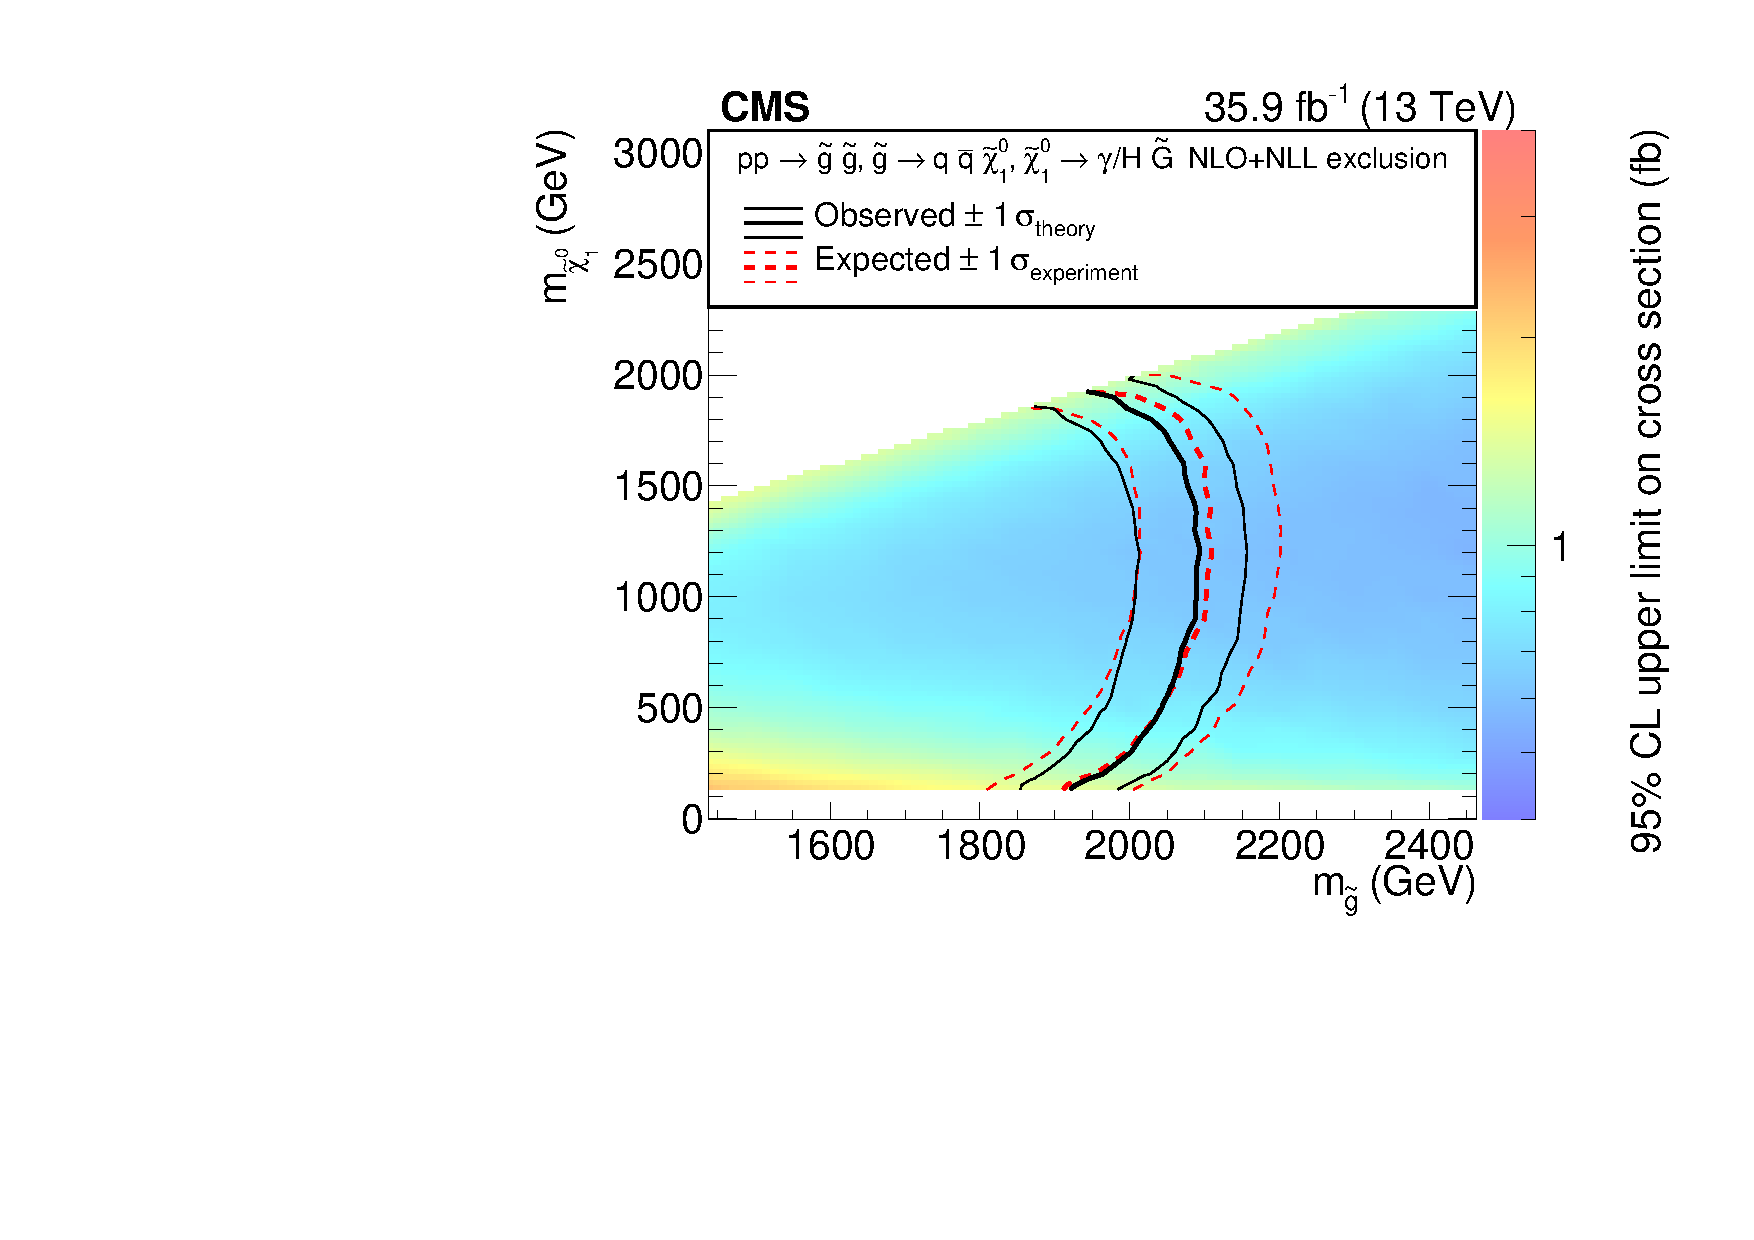
\includegraphics[width=0.48\linewidth]{../Figures/Chap4/Figure_005-a.pdf}
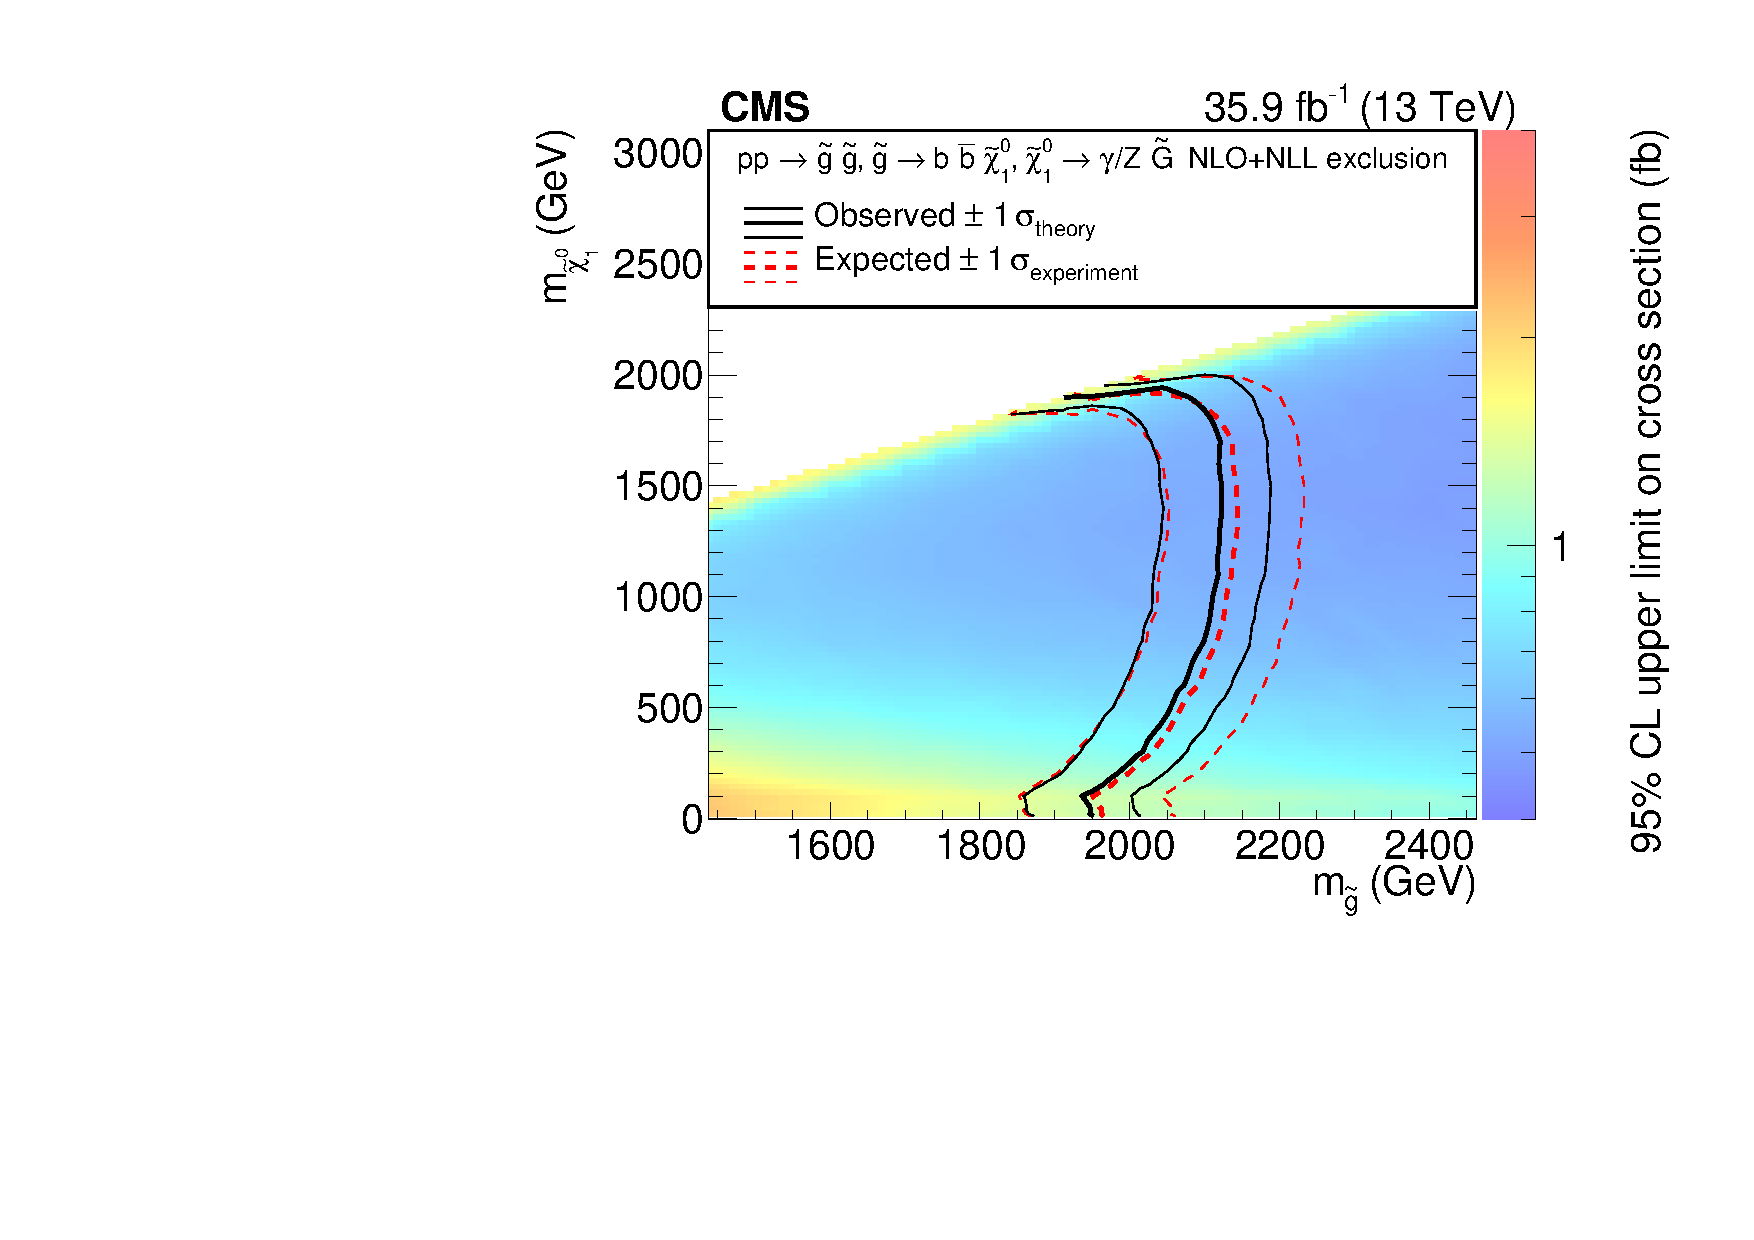
\includegraphics[width=0.48\linewidth]{../Figures/Chap4/Figure_005-b.pdf}\\
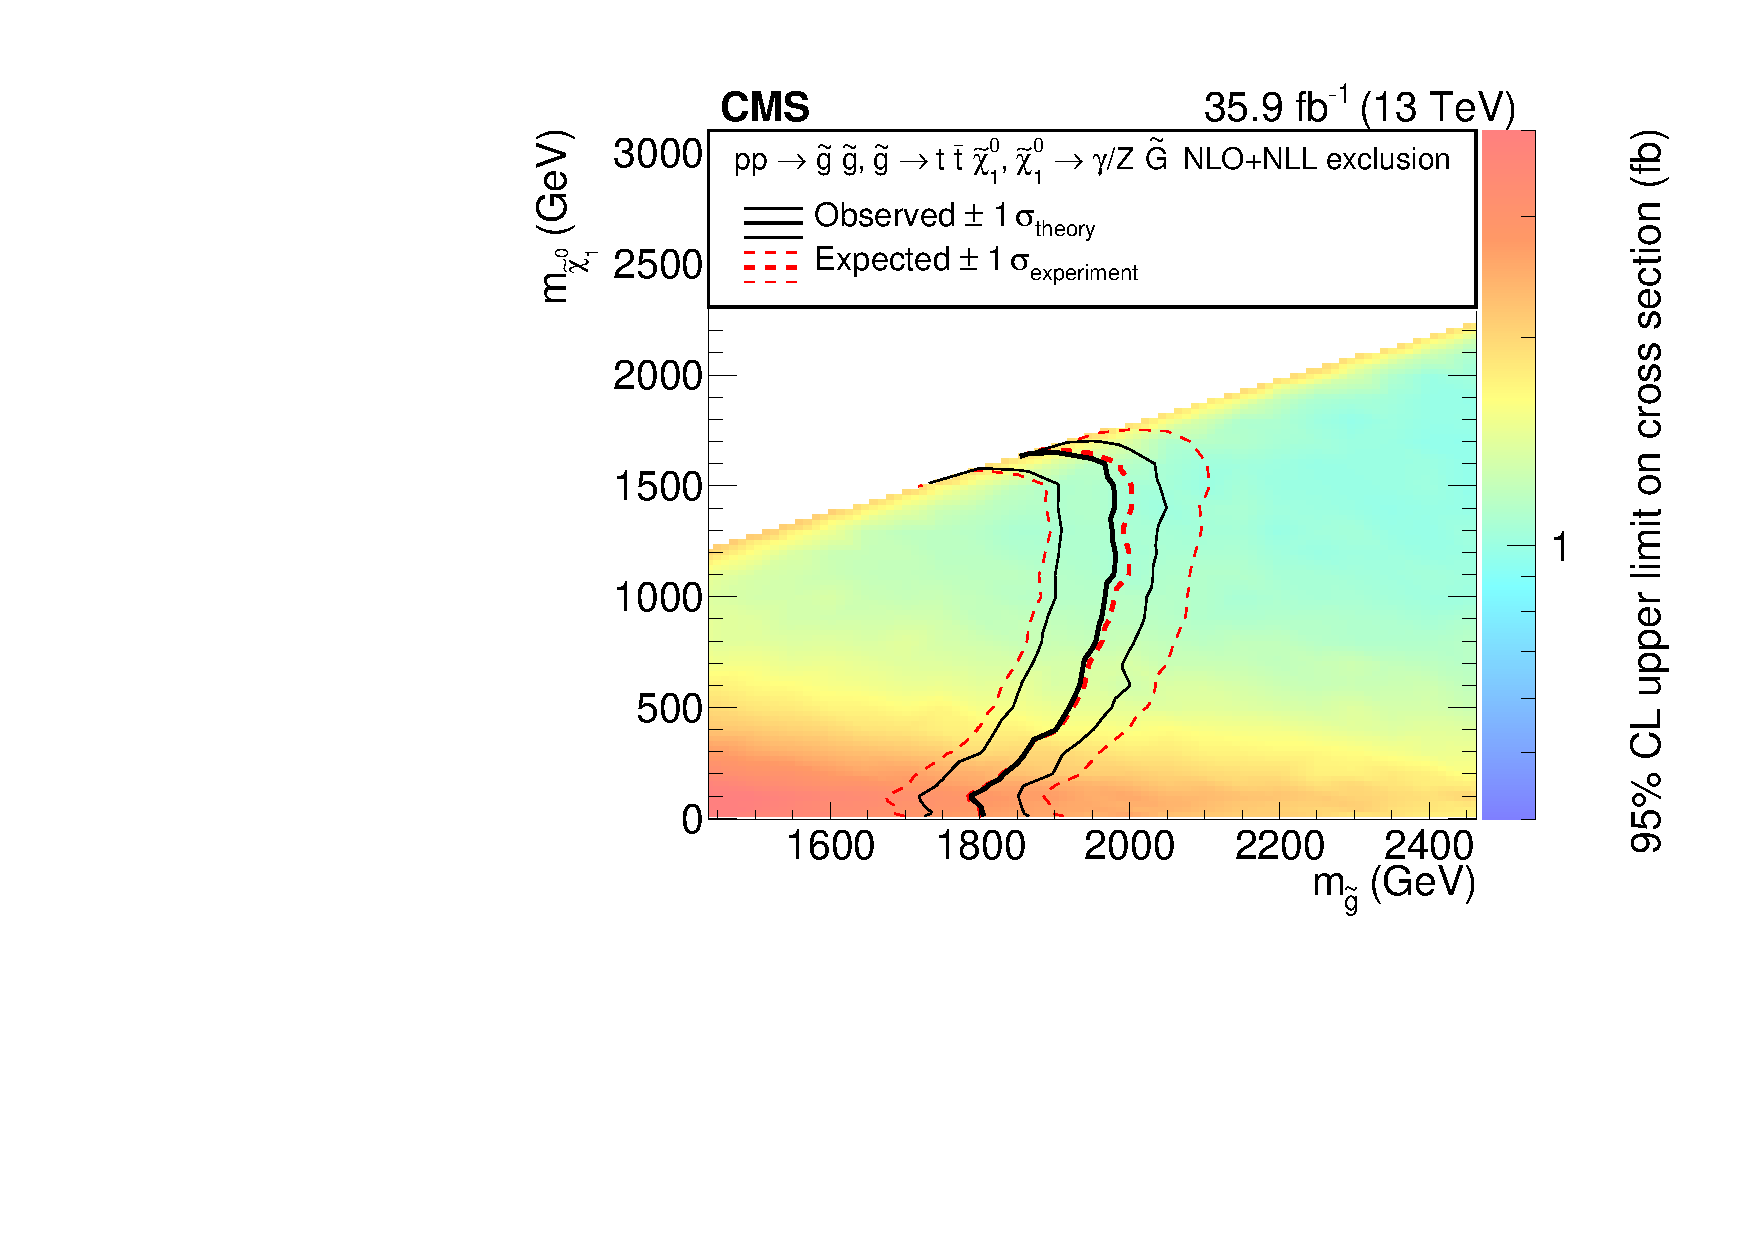
\includegraphics[width=0.48\linewidth]{../Figures/Chap4/Figure_005-c.pdf}
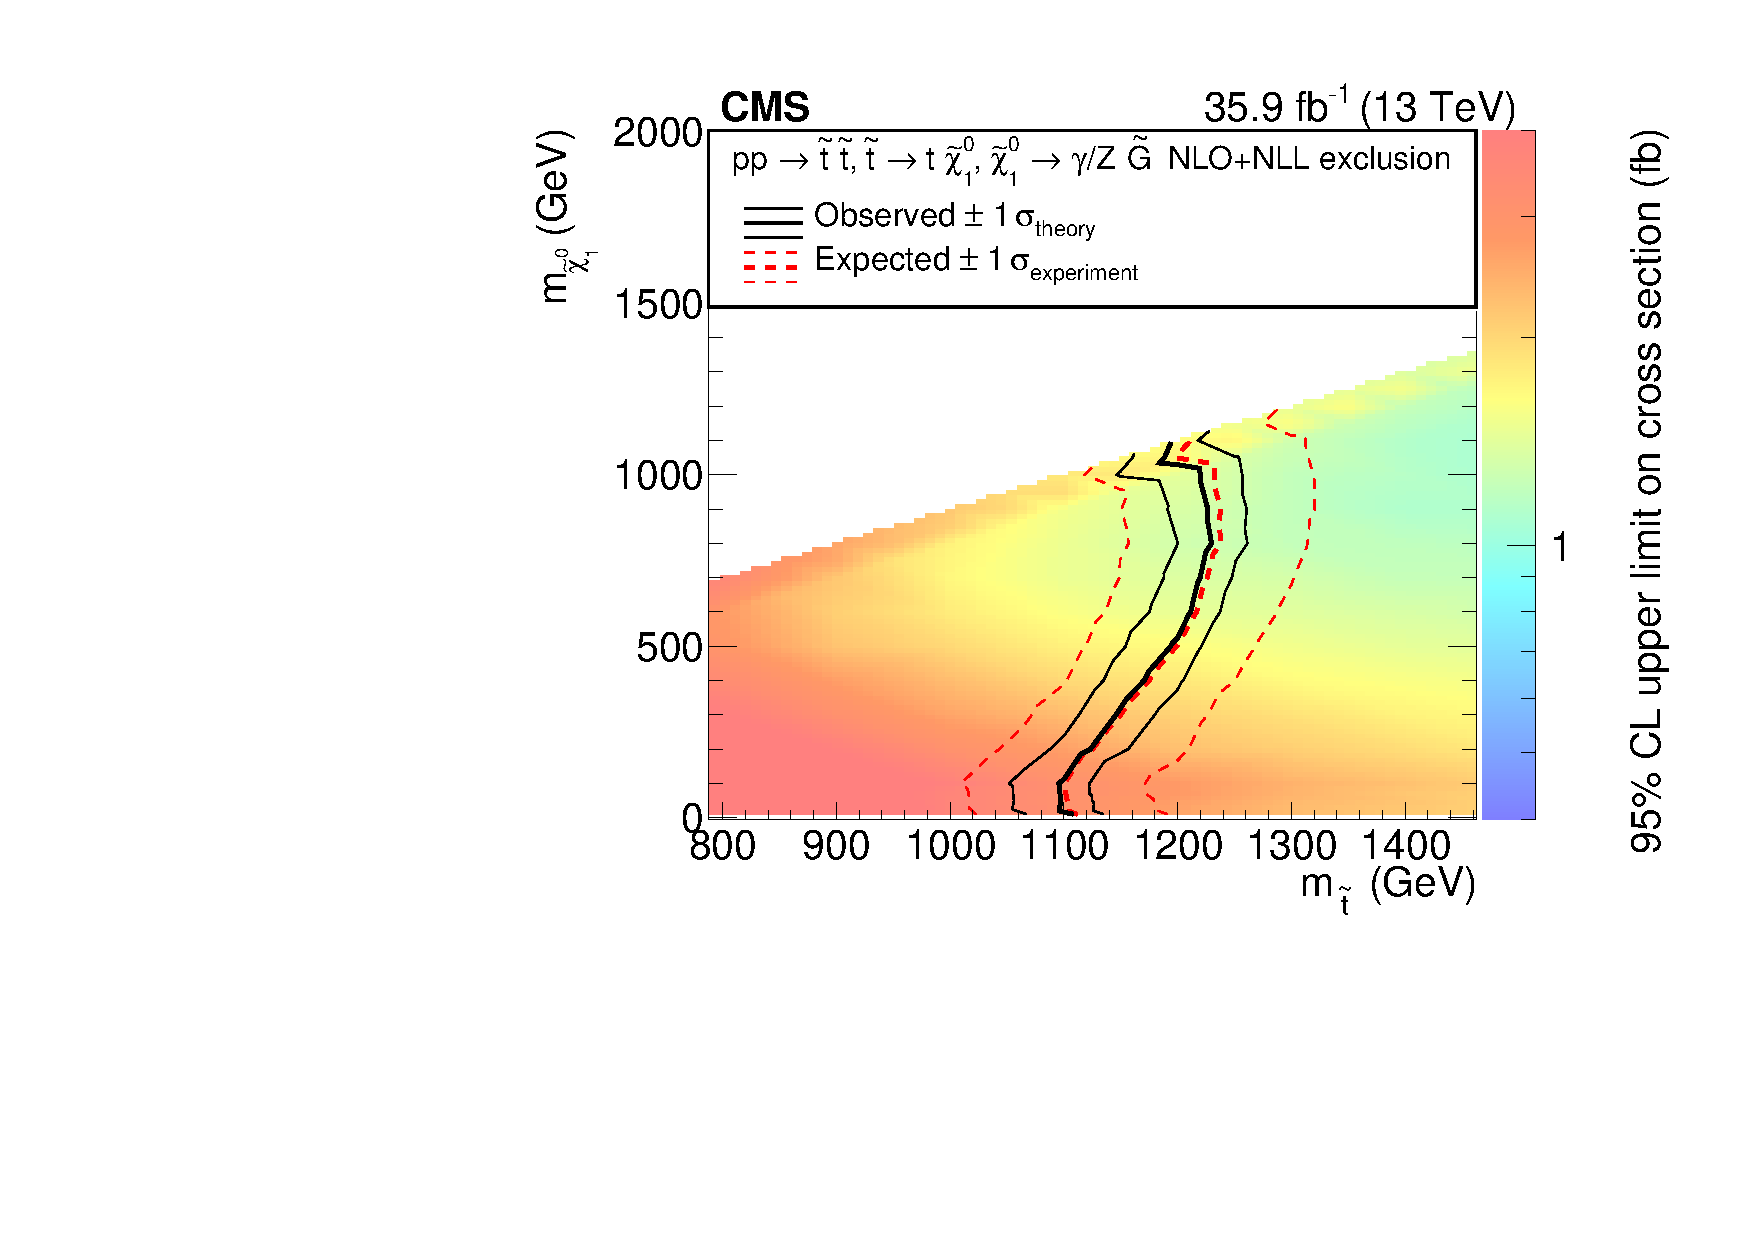
\includegraphics[width=0.48\linewidth]{../Figures/Chap4/Figure_005-d.pdf}
\captionsetup{width=.95\linewidth}
\caption{Observed and expected 95\% CL upper limits for gluino or top squark pair production cross sections
for the T5qqqqHG (upper left), T5bbbbZG (upper right), T5ttttZG (bottom left), and T6ttZG
(bottom right) models. Black lines denote the
observed exclusion limit and the uncertainty due to variations of the
theoretical prediction of the gluino or top squark pair production cross section.
The dashed lines correspond to the region containing 68\% of the distribution of
the expected exclusion limits under the background-only hypothesis.}
\label{fig:exclusions}
\end{figure*}

Generally, the limits degrade at both high and low $\mnlsp$.
For $\mnlsp\approx \mgluino\,(\mstop)$, the quarks from the decay of gluinos (top squarks) have low \pt.
Correspondingly, the \htg, \nj, and \nb distributions tend toward lower values, reducing the signal efficiency and causing
signal events to populate regions with higher background yields. For small $\mnlsp$,
the quarks produced in the decay of gluinos or top squarks have high \pt but lower \ptmiss on average.
For all models except T5qqqqHG, when the NLSP mass drops below the mass of the
Z boson, the kinematics of the NLSP decay require the Z boson to be far off-shell.
As the Z boson mass is forced to be lower, the LSP will carry a larger fraction of the momentum of the NLSP, producing larger \ptmiss.
This causes a slight increase in the sensitivity when the NLSP mass is near the Z boson mass.
While a similar effect would happen for the T5qqqqHG model,
the simulation used here does not probe the region of parameter space where the Higgs boson
would be forced to have a mass far off-shell.

The features seen in exclusion curves can be understood using acceptance $\times$ efficiency plots shown in figure \ref{fig:sigEff} in Appendix \ref{sec:SigAccEff}.

\begin{sloppypar} For moderate \mnlsp, gluino masses as large as 2090, 2120, and 1970 \GeV are excluded for the T5qqqqHG, T5bbbbZG, and T5ttttZG models, respectively.
Top squark masses as large as 1230 \GeV are excluded for the T6ttZG model.
For small \mnlsp, gluino masses as large as 1920, 1950, and 1800 \GeV are excluded for the T5qqqqHG, T5bbbbZG, and T5ttttZG models, respectively.
Top squark masses as large as 1110 \GeV are excluded for the T6ttZG model.
There is close agreement between the observed and expected limits.
\end{sloppypar}

\section{Summary}
\label{sec:summary}

\begin{sloppypar} A search for gluino and top squark pair production is presented, based on a proton-proton collision
dataset at a center-of-mass energy of 13 TeV recorded with the CMS detector in 2016.
The data correspond to an integrated luminosity of 35.9\fbinv.  Events are
required to have at least one
isolated photon with transverse momentum ${\pt>100\ \gev}$, two jets with ${\pt>30\ \gev}$ and pseudorapidity ${|\eta|<2.4}$,
and missing transverse momentum ${\ptmiss>200\ \gev}$.
\end{sloppypar}

The data are categorized into 25 exclusive signal regions based on the number of
jets, the number of {\cPqb}-tagged jets, and \ptmiss.  Background yields from the standard model
processes are predicted using simulation and data control regions.  The observed event
yields are found to be consistent with expectations from the standard model processes
within the uncertainties.

Results are interpreted in the context of simplified models.  Four such models
are studied, three of which involve gluino pair production
and one of which involves top squark pair production. All models assume
a gauge-mediated supersymmetry (SUSY) breaking scenario, in which the lightest SUSY particle is a gravitino (\PXXSG).
We consider scenarios in which the gluino decays to
a neutralino \PSGczDo and a pair of light-flavor quarks (T5qqqqHG),
bottom quarks (T5bbbbZG), or top quarks (T5ttttZG).
In the T5qqqqHG model, the \PSGczDo decays with equal probability either to a photon and a \PXXSG
or to a Higgs boson and a \PXXSG.  In the T5bbbbZG
and T5ttttZG models, the \PSGczDo decays with equal probability either to a photon and a \PXXSG or to a
Z boson and a \PXXSG.  In the top squark pair production model (T6ttZG),
top squarks decay to a top quark and \PSGczDo, and the \PSGczDo decays with equal probability either to a photon and a \PXXSG or to a Z boson and a \PXXSG.

Using the cross sections for SUSY pair production
calculated at next-to-leading order plus next-to-leading logarithmic accuracy, we place 95\% confidence level lower limits on
the gluino mass as large as 2120 \gev, depending on the model and the \mnlsp value, and
limits on the top squark mass as large as 1230 \gev, depending on the \mnlsp value.
These results significantly improve upon those from previous searches for SUSY with photons.

\section{Outlook}
\label{sec:outlook}
The main focus of this search was on GMSB scenarios with strong production of gluinos and stops.
However, this is a generic search which searches for any beyond SM phenomena resulting in events
with photon, \ptmiss, \nj and \nb final states. It is also possible to use the results of this search 
interpret them in terms of any other models. In this section we study the scope of this search by considering 
EW production of SUSY particles with SMS scenarios.
\subsection{Electroweak models}
Two kinds of electroweak (EWK) SMS scenarios, TChiWG and TChiNG, are studied and the expected limits are determined.
In TChiWG (Figure \ref{fig:CMS-SUS-16-046_Figure_001} top), there is production of neutralinos (\PSGczDo) and charginos (\PSGczDq).
The decay of \PSGczDo gives $\grav + \gamma$ and the decay of \PSGczDq gives $\mathrm{W^\pm}+\grav$. In TChiNG (Figure \ref{fig:CMS-SUS-16-046_Figure_001} bottom) scenario, \PSGczDq and \PSGczDo are nearly mass degenerate, with \PSGczDq being slightly
heavier than \PSGczDo and its decay gives rise to \PSGczDo and soft particles which generally do not pass object level requirements. In this case, two production modes, \PSGczDq-\PSGczDq (bottom left) and \PSGczDq-\PSGczDo (bottom right) are considered. The branching fraction for the decay of \PSGczDo is 50\% $\grav + \gamma$, 25\% $\grav + $H and 25\% $\grav +$Z. These are the same models as considered by the electrowikino search performed by CMS in Ref. \cite{Sirunyan:2017nyt}. The cross sections are calculated at NLO+NLL accuracy \cite{Fuks:2013vua,Fuks:2012qx,Beenakker:1999xh} and are computed in the limit of mass degenerate wino $\tilde{\chi}_{2}^{0}$ and \PSGczDq.
\begin{figure}[h!]
\centering
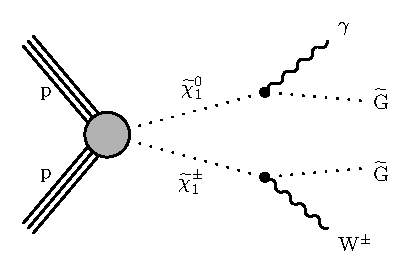
\includegraphics[width=0.48\linewidth]{../Figures/Chap4/CMS-SUS-16-046_Figure_001-b}\\
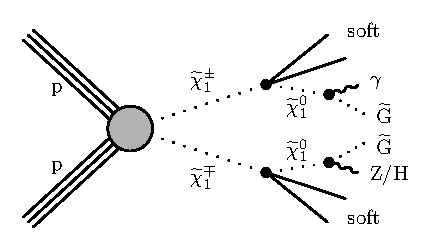
\includegraphics[width=0.48\linewidth]{../Figures/Chap4/CMS-SUS-16-046_Figure_001-c}
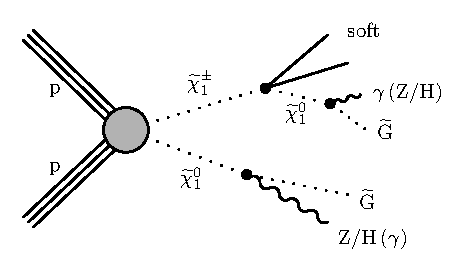
\includegraphics[width=0.48\linewidth]{../Figures/Chap4/CMS-SUS-16-046_Figure_001-d}
\caption[TChiWG and TChiNG SMS digrams]{SMS diagrams for TChiWG (top) and TChiNG (bottom).}
\label{fig:CMS-SUS-16-046_Figure_001}
\end{figure}
\subsection{Sensitivity of the search}
The results of the search described in this thesis are interpreted in terms of the above mentioned SMS scenarios and 
the expected limits on the cross section are compared with Ref. \cite{Sirunyan:2017nyt}. Figure \ref{fig:limitPlotter_EW}
shows the expected upper limits on the cross section for TChiWG scenario (left) and TChiNG (right) scenario using this search.

\begin{figure}[h!]
\centering
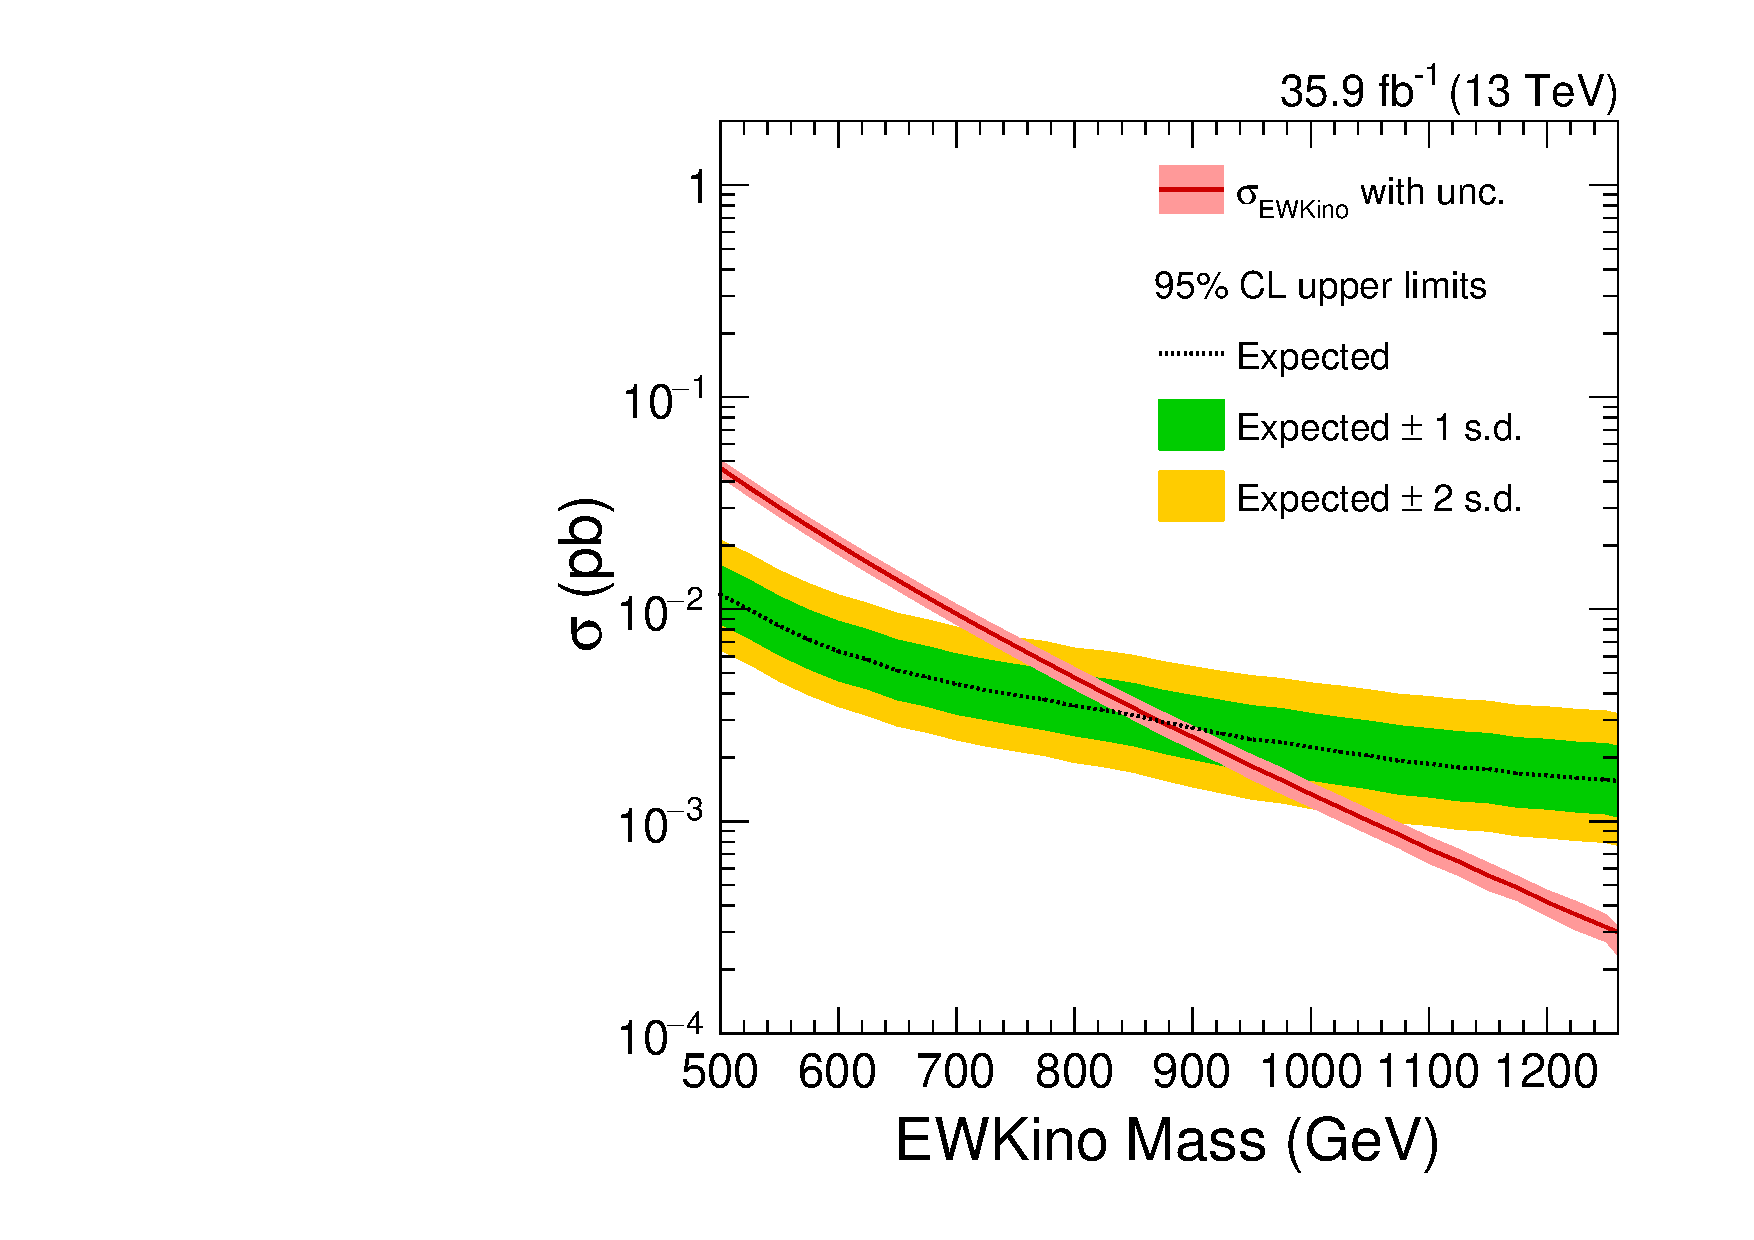
\includegraphics[width=0.48\linewidth]{../Figures/Chap4/limitPlotter_TChiWG}
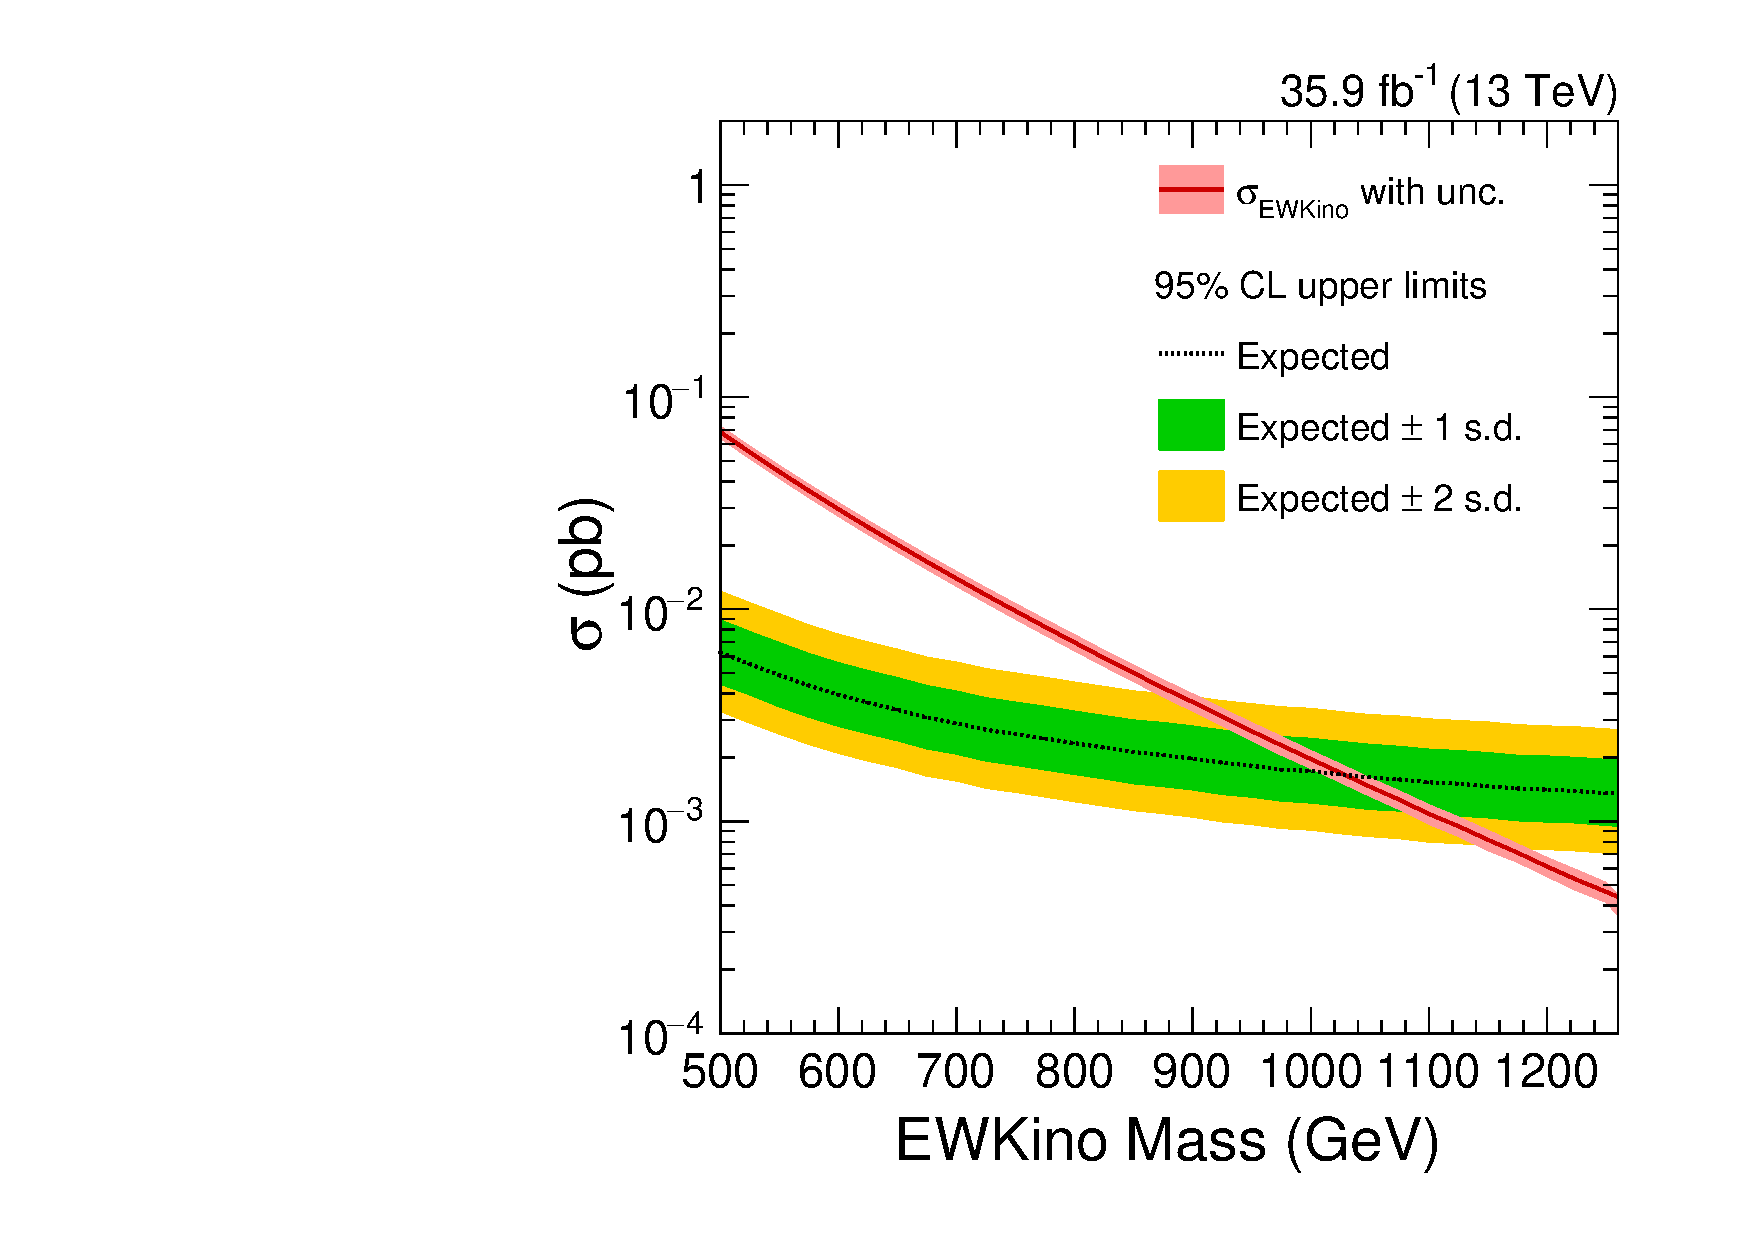
\includegraphics[width=0.48\linewidth]{../Figures/Chap4/limitPlotter_TChiNG}
\caption[Expected UL for EW for SUSY]{Expected upper limit on the cross section of TChiWG (left) and TChiNG (right) models.}
\label{fig:limitPlotter_EW}
\end{figure}
EWKino masses below 870 \gev for TChiWG case and mass below 1030 \gev for TChiNG case can be excluded. 
The EW search of CMS \cite{Sirunyan:2017nyt} has expected 
EWKino mass exclusion of 920 \gev and 1070 \gev for TChiWG and TChiNG models respectively, which is about 40-50 \gev higher than
this search. 

It is also worth noting that the search described in this thesis does not consider all sources of systematic uncertainties
in EWKino signal models. Only the statistical uncertainty in the MC samples and integrated luminosity uncertainty are considered.
If all the sources of systematic uncertainty are considered, the limits in this search are going to degrade to some extent. However,
these studies lead to an important conclusion that the search can target a wide range of models although strong production scenarios
were the main focus.

One of the possible ways to improve this search and have a good sensitivity for EW models, is to loosen hadronic activity criteria 
mentioned in section \ref{sec:event-selection}. At present, the search requires minimum \ST (sum \pt of jets and photon) of 500 \gev,
which is very disadvantageous for EWKino production models. One possible way to reduce the background in low \ST regions, is increasing
\ptg or \ptmiss threshold.

During run 2 (year 2016-2018), CMS has collected more than 135 \fbinv of data and this is going to be an advantage for EW SUSY
searches. A combination of several searches with photons is performed by CMS using 2016 data \textcolor{red}{Add ref for GGM PAS}.
This combination uses photon + \ST search \cite{Sirunyan:2017yse}, EW search \cite{Sirunyan:2017nyt}, photon + lepton search
\cite{Sirunyan:2018psa} and diphoton search \textcolor{red}{Add ref for diphoton PAS}. Since this search has very good sensitivity 
for strong SUSY production models, and if one performs further optimization the search for EW SUSY models, this search is going to play
a significant role on the path to discovery or to constrain SUSY models.